% Created 2017-06-05 Mon 12:47
% Intended LaTeX compiler: pdflatex
\documentclass[presentation]{beamer}
\usepackage[utf8]{inputenc}
\usepackage[T1]{fontenc}
\usepackage{graphicx}
\usepackage{grffile}
\usepackage{longtable}
\usepackage{wrapfig}
\usepackage{rotating}
\usepackage[normalem]{ulem}
\usepackage{amsmath}
\usepackage{textcomp}
\usepackage{amssymb}
\usepackage{capt-of}
\usepackage{hyperref}
\usetheme{default}
\author{Kevin Caye\(^{1}\), Olivier Michel\(^{2}\), Jean-Luc Bosson\(^{1}\), Olivier Francois\(^{1}\)}
\date{2017-01-06}
\title{Matrix factorization methods for association mapping}
\institute{$^{1}$ TIMC-IMAG, $^{2}$ GIPSA-lab}
\usebackgroundtemplate{
\includegraphics[width=\paperwidth]{background.pdf}}%
\addtobeamertemplate{frametitle}{\vskip2ex}{}
\newcommand{\matr}[1]{\mathbf{#1}} %% \matr{}
\newcommand{\G}{\matr{G}} %% \G 
\newcommand{\U}{\matr{U}} %% \U
\newcommand{\V}{\matr{V}} %% \V
\newcommand{\X}{\matr{X}} %% \X
\newcommand{\B}{\matr{B}} %% \B
\newcommand{\E}{\matr{E}} %% \E
\newcommand{\C}{\matr{C}} %% \C
\newcommand{\PP}{\matr{P}} %% \PP
\newcommand{\Id}{\matr{Id}} %% \Id
\newcommand\norm[1]{\left\lVert#1\right\rVert} %% \norm
\newcommand{\pvalue}{$p$-value} %% \pvalue

\thankstitle{Thank you!}
\hypersetup{
 pdfauthor={Kevin Caye\(^{1}\), Olivier Michel\(^{2}\), Jean-Luc Bosson\(^{1}\), Olivier Francois\(^{1}\)},
 pdftitle={Matrix factorization methods for association mapping},
 pdfkeywords={},
 pdfsubject={},
 pdfcreator={Emacs 25.1.1 (Org mode 9.0.3)}, 
 pdflang={English}}
\begin{document}

\maketitle
\begin{frame}{Outline}
\tableofcontents
\end{frame}


\section{Introduction}
\label{sec:org7357c21}

\begin{frame}[label={sec:org7768154}]{Dataset}
\alert{Dataset}
\begin{itemize}
\item \(\Y\) output observed matrix
\item \(\X\) primary variables matrix.
\end{itemize}

\alert{We want} to detect output variables which are in relationship with the primary
interest variable.

\alert{Example}
\begin{itemize}
\item Association of DNA methylation with Rheumatoid Arthritis (RA) \cite{Liu_2013}
\begin{itemize}
\item \(\Y\) records DNA methylation level for \(\Yrow = 689\) at \(\Ycol = 162~038\)
sites
\item \(\X\) records RA disease state for each individual.
\end{itemize}
\end{itemize}
\end{frame}

\begin{frame}[label={sec:org0bcc100}]{Multiple Hypothesis Testing: Simple Linear Regression}
Linear model suppose that
    $$\Y =  \X \B^{T} + \E$$
  where
\begin{itemize}
\item \(\B\) is the primary effect matrix
\item \(\E\) is the residual error matrix.
\end{itemize}

We want to detect \(j\) variable where we can reject the hypothesis 

$$ H_0: \B_j = 0.$$
\end{frame}

\begin{frame}[label={sec:org3cb5052}]{Example: Linear Regression on RA Dataset}
\begin{center}
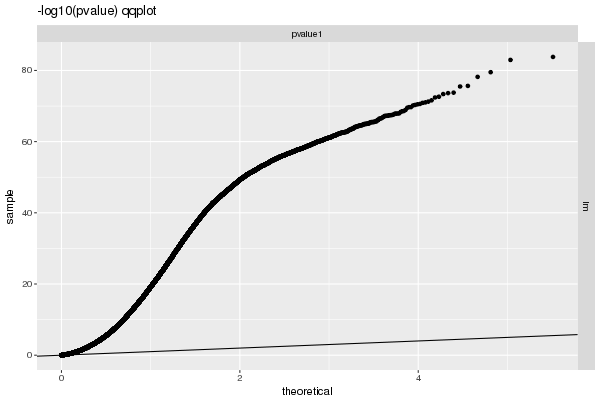
\includegraphics[width=.9\linewidth]{./Rplots/GSE42861_qqplot_lm.png}
\end{center}
\end{frame}

\begin{frame}[label={sec:orgc9bdf17}]{Example: Principal Component Analysis of RA dataset}
\begin{center}
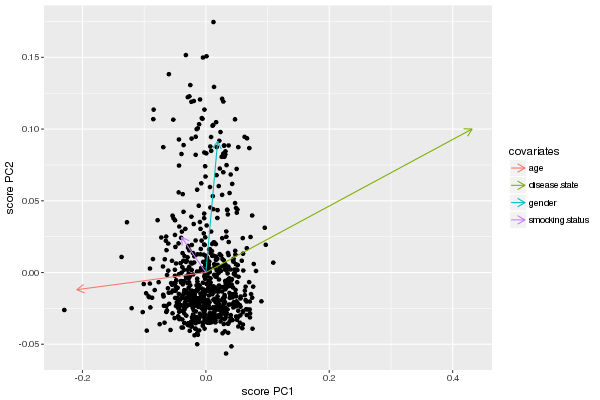
\includegraphics[width=.9\linewidth]{./Rplots/PC_RA.png}
\end{center}
\end{frame}

\section{Latent factor in Multiple Hypothesis Testing}
\label{sec:org2acb210}
\begin{frame}[label={sec:org93b6ce7}]{Latent Factor Mixed Model}
Following the common notation in \alert{latent factor mixed model} (LFMM) we write the following
model \cite{wang2015confounder,frichot13_testin_assoc_between_loci_envir}

\begin{equation}
\label{eq:model}
\Y = \X \B^T + \U \V^T + \E 
\end{equation}

\begin{itemize}
\item \(\U \V^{T}\) is the unwanted variation
\item \(\X \B^{T}\) is the variation of interest
\item \(\E\) the residual noise.
\end{itemize}
\end{frame}

\begin{frame}[label={sec:org65ba035}]{Estimation}
\alert{L2-norm loss function}
\begin{equation*}
\label{eq:optim_no_reg}
\LfmmL
\end{equation*}
\alert{The problem} is \(L\) do not allow to separate source of unwanted variation from
interest variation.
\begin{equation*}
L(\U, \V, \B) = L(\U - \X \matr{C}, \V, \B + \V \matr{C}^{T})
\end{equation*}
\end{frame}
\begin{frame}[label={sec:org096be5a}]{Regularized estimation}
\alert{Ridge} regularized LFMM

\begin{equation*}
\LfmmLridge
\end{equation*}

\alert{Lasso} regularized LFMM

\begin{equation*}
L_{lasso}(\C, \B) =  \frac{1}{2} \norm{\Y - \C - \X \B^T}_{F}^2 + \lambda \norm{\B}_{1} + \gamma \norm{\C}_{*}
\end{equation*}

where $$\C = \U \V^{T}.$$
\end{frame}

\section{Some results}
\label{sec:org64f75ee}
\begin{frame}[label={sec:org9b5e6d5}]{Numerical validation}
We performed simulations of LFMM generative model $$\Y = \X \B^T + \U \V^T + \E$$ 

with $$ B_{j} \neq 0$$ for some variables associated with the variable of
interest \(\X\).
\end{frame}
\begin{frame}[label={sec:org76bf15a}]{Numerical validation}
\begin{center}
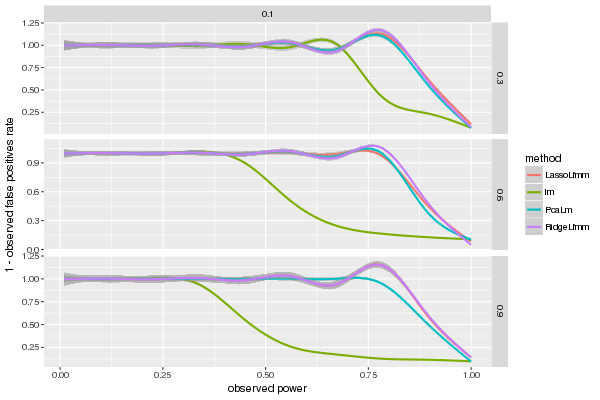
\includegraphics[width=.9\linewidth]{./Rplots/method_comp.png}
\end{center}
\end{frame}

\begin{frame}[label={sec:org705f355}]{AR dataset}
We retrieve main site found in other study using explicitly confounding
variables (age, gender, smoking status, cellular composition).
\end{frame}

\begin{frame}[label={sec:org7ec42ef}]{Thank you !}
Thank you for your attention ! 
\end{frame}

\begin{frame}[label={sec:orgdc978db}]{References}
\bibliography{../../../biblio}
\bibliographystyle{apalike}
\end{frame}
\end{document}